\documentclass{standalone}
\usepackage{mintikz}

\pgfdeclarelayer{background}
\pgfdeclarelayer{foreground}
\pgfsetlayers{background,main,foreground}
\usepackage{pifont}% http://ctan.org/pkg/pifont
\newcommand{\cmark}{\ding{51}}%
\newcommand{\xmark}{\ding{55}}%

\begin{document}
\thispagestyle{empty}
\begin{tikzpicture}[]
    %\draw[thin, black!20] (0,0) grid (20,-20);
    \tikzset{header/.style={draw, rounded corners, fill=#1!30},
    header/.default={gray}}
    % Start left
    \begin{scope}[local bounding box=PRIORBOX, yshift=0cm]
        %%%%%%%%%%%%%%%%%%%%%%%%%%%%%%%%%%%%%%%%%%%%%%%%%%%%%%%%%%%%%%%%%%%%%%%
        % Start PRIOR
        \node[] (PRIOR) at (0,0) {};
        %%%%%%%%%%%%%%%%%%%%%%%%%%%%%%%%%%%%%%%%%%%%%%%%%%%%%%%%%%%%%%%%%%%%%%%
        % Start SIMLIM
        \node[header=black, below=20pt]
            (SIMLIB) at (PRIOR.south) {SIMLIB};
        \matrix[matrix of nodes, anchor=north,
            row sep=-1pt, column sep=-\pgflinewidth,
            text width=40pt, align=center,
            %left delimiter=|,
            nodes={anchor=center, align=center}]
            (Msimlib) at ([shift={(0,-0.1)}]SIMLIB.south)
            {$z$ & Date & RADEC \\
            \vdots & \vdots & \vdots \\};
        % Vlines
        \foreach \n in {1, 2}{
        \draw[]
            (Msimlib-1-\n.north east-|Msimlib-2-\n.south east) |-
        (Msimlib-2-\n.south east);}
        %%%%%%%%%%%%%%%%%%%%%%%%%%%%%%%%%%%%%%%%%%%%%%%%%%%%%%%%%%%%%%%%%%%%%%%
        % START HOSTLIB
        \node[header=black, below=12pt]
            (HOSTLIB) at (Msimlib.south) {HOSTLIB};
        \matrix[matrix of nodes, anchor=north,
            row sep=-1pt, column sep=-\pgflinewidth,
            text width=40pt, align=center,
            %left delimiter=|,
            nodes={anchor=center, align=center}]
            (Mhostlib) at ([shift={(0,-0.1)}]HOSTLIB.south)
            {ID & $z$ & hostmass & $x_1$ & $c$ & $\Delta$ mag \\
            \vdots & \vdots & \vdots & \vdots & \vdots & \vdots\\
            \vdots & \vdots & \vdots & \vdots & \vdots & \vdots\\};
        % Vlines
        \foreach \n in {1, 3, 4, 5}{
        \draw[]
            (Mhostlib-1-\n.north east-|Mhostlib-3-\n.south east) |-
        (Mhostlib-3-\n.south east);}
        \draw[]
            (Mhostlib-2-2.north east-|Mhostlib-3-2.south east) |-
            (Mhostlib-3-2.south east);
        %%%%%%%%%%%%%%%%%%%%%%%%%%%%%%%%%%%%%%%%%%%%%%%%%%%%%%%%%%%%%%%%%%%%%%%
        % SIMLIB to HOSTLIB
        \draw[->]
            (Msimlib-2-1) to[bend right]
            (Mhostlib-1-2);
        % HOSTLIB z to hostmass
        \draw[->]
            ([shift={(3pt,0)}]Mhostlib-1-2.center) --
            ([shift={(-21pt,0)}]Mhostlib-1-3.center);
        %%%%%%%%%%%%%%%%%%%%%%%%%%%%%%%%%%%%%%%%%%%%%%%%%%%%%%%%%%%%%%%%%%%%%%%
        % WGTMAP
        \pgfplotstableread{../data/SDSS.txt}{\wgttable}
        \node[header=black, below=20pt]
            (WEIGTHMAP) at (Mhostlib.south) {WEIGTHMAP};
        \begin{axis}[
            shift={($(WEIGTHMAP.south)+(0,-8pt)$)},
            anchor=north,
            xmin=8, xmax=12.3,
            ymin=0, ymax=1,
            xlabel=$M_{\rm host}$, ylabel=$P(M)$,
            axis lines=left,
            clip=false]
            \addplot[black, samples=500]
                table[x=M, y=WGT] from \wgttable;
        \end{axis}
        % \coordinate (XS1) at (SIMLIB.east-|Mhostlib-1-6.east);
        % \len{(XS1)}{(SIMLIB.center)}{\xsa}
        % \node[] at (3,0) {\Huge \xsa};
    \end{scope}
    %%%%%%%%%%%%%%%%%%%%%%%%%%%%%%%%%%%%%%%%%%%%%%%%%%%%%%%%%%%%%%%%%%%%%%%
    \begin{scope}[local bounding box=TRUEBOX, xshift=8cm, at=(PRIOR)]
    %%%%%%%%%%%%%%%%%%%%%%%%%%%%%%%%%%%%%%%%%%%%%%%%%%%%%%%%%%%%%%%%%%%%%%%
        % Start TRUE
        \node[header=orchid] (TRUE) at (3,0) {V\'ERIT\'E};
        %%%%%%%%%%%%%%%%%%%%%%%%%%%%%%%%%%%%%%%%%%%%%%%%%%%%%%%%%%%%%%%%%%%%%%%
        % M DIST from BP_lowz HOSTLIB
        \pgfplotstableread{../data/mdist.txt}{\mtable}
        \begin{axis}[name=mdist, scale=0.5,
            yshift=-1cm, anchor=north,
            xmin=6, xmax=14,
            ymin=0, ymax=0.6,
            xlabel=$M$, ylabel=$P$,
            axis lines=left,
            clip=false]
            \addplot[smooth, black]
                table[x=M, y=P] from \mtable;
        \end{axis}
        %%%%%%%%%%%%%%%%%%%%%%%%%%%%%%%%%%%%%%%%%%%%%%%%%%%%%%%%%%%%%%%%%%%%%%%
        % X1 DIST from basemodel
        \pgfplotstableread{../data/basemodel.txt}{\basetable}
        \begin{axis}[name=x1dist, scale=0.5,
            at={(mdist.below south west)}, yshift=-0.3cm, anchor=north west,
            xmin=-3, xmax=3,
            ymin=0, ymax=0.5,
            xlabel=$\bar{x_1}$, ylabel=$P$,
            axis lines=left,
            clip=false]
            \addplot[smooth, black]
                table[x=xlin, y=values] from \basetable;
        \end{axis}
        %%%%%%%%%%%%%%%%%%%%%%%%%%%%%%%%%%%%%%%%%%%%%%%%%%%%%%%%%%%%%%%%%%%%%%%
        % c DIST from stretchevol's asym with Scolnic 18 params:
        % -0.068, 0.034, 0.123
        \pgfplotstableread{../data/casym.txt}{\ctable}
        \begin{axis}[name=cdist, scale=0.5,
            at={(x1dist.below south west)}, yshift=-0.3cm, anchor=north west,
            xmin=-0.3, xmax=0.3,
            ymin=0, ymax=5,
            xlabel=$\bar{c}$, ylabel=$P$,
            axis lines=left,
            clip=false]
            \addplot[smooth, black]
                table[x=clin, y=values] from \ctable;
        \end{axis}
        %%%%%%%%%%%%%%%%%%%%%%%%%%%%%%%%%%%%%%%%%%%%%%%%%%%%%%%%%%%%%%%%%%%%%%%
        % z DIST Rate from equation 6 of DES 2019
        % https://arxiv.org/pdf/1811.02379.pdf
        \begin{axis}[name=zdist, scale=0.5,
            at={(cdist.below south west)}, yshift=-0.3cm, anchor=north west,
            xmin=0, xmax=1.2,
            ymin=0, ymax=7.5,
            xlabel=$\bar{z}$, ylabel=\# (1$^{-15}$),
            axis lines=left,
            clip=true]
            \addplot[smooth, black]
                {1.75*(1+x)^2.11};
        \end{axis}
        \node[right] (TS) at ([shift={(1,0)}]cdist.east)
            {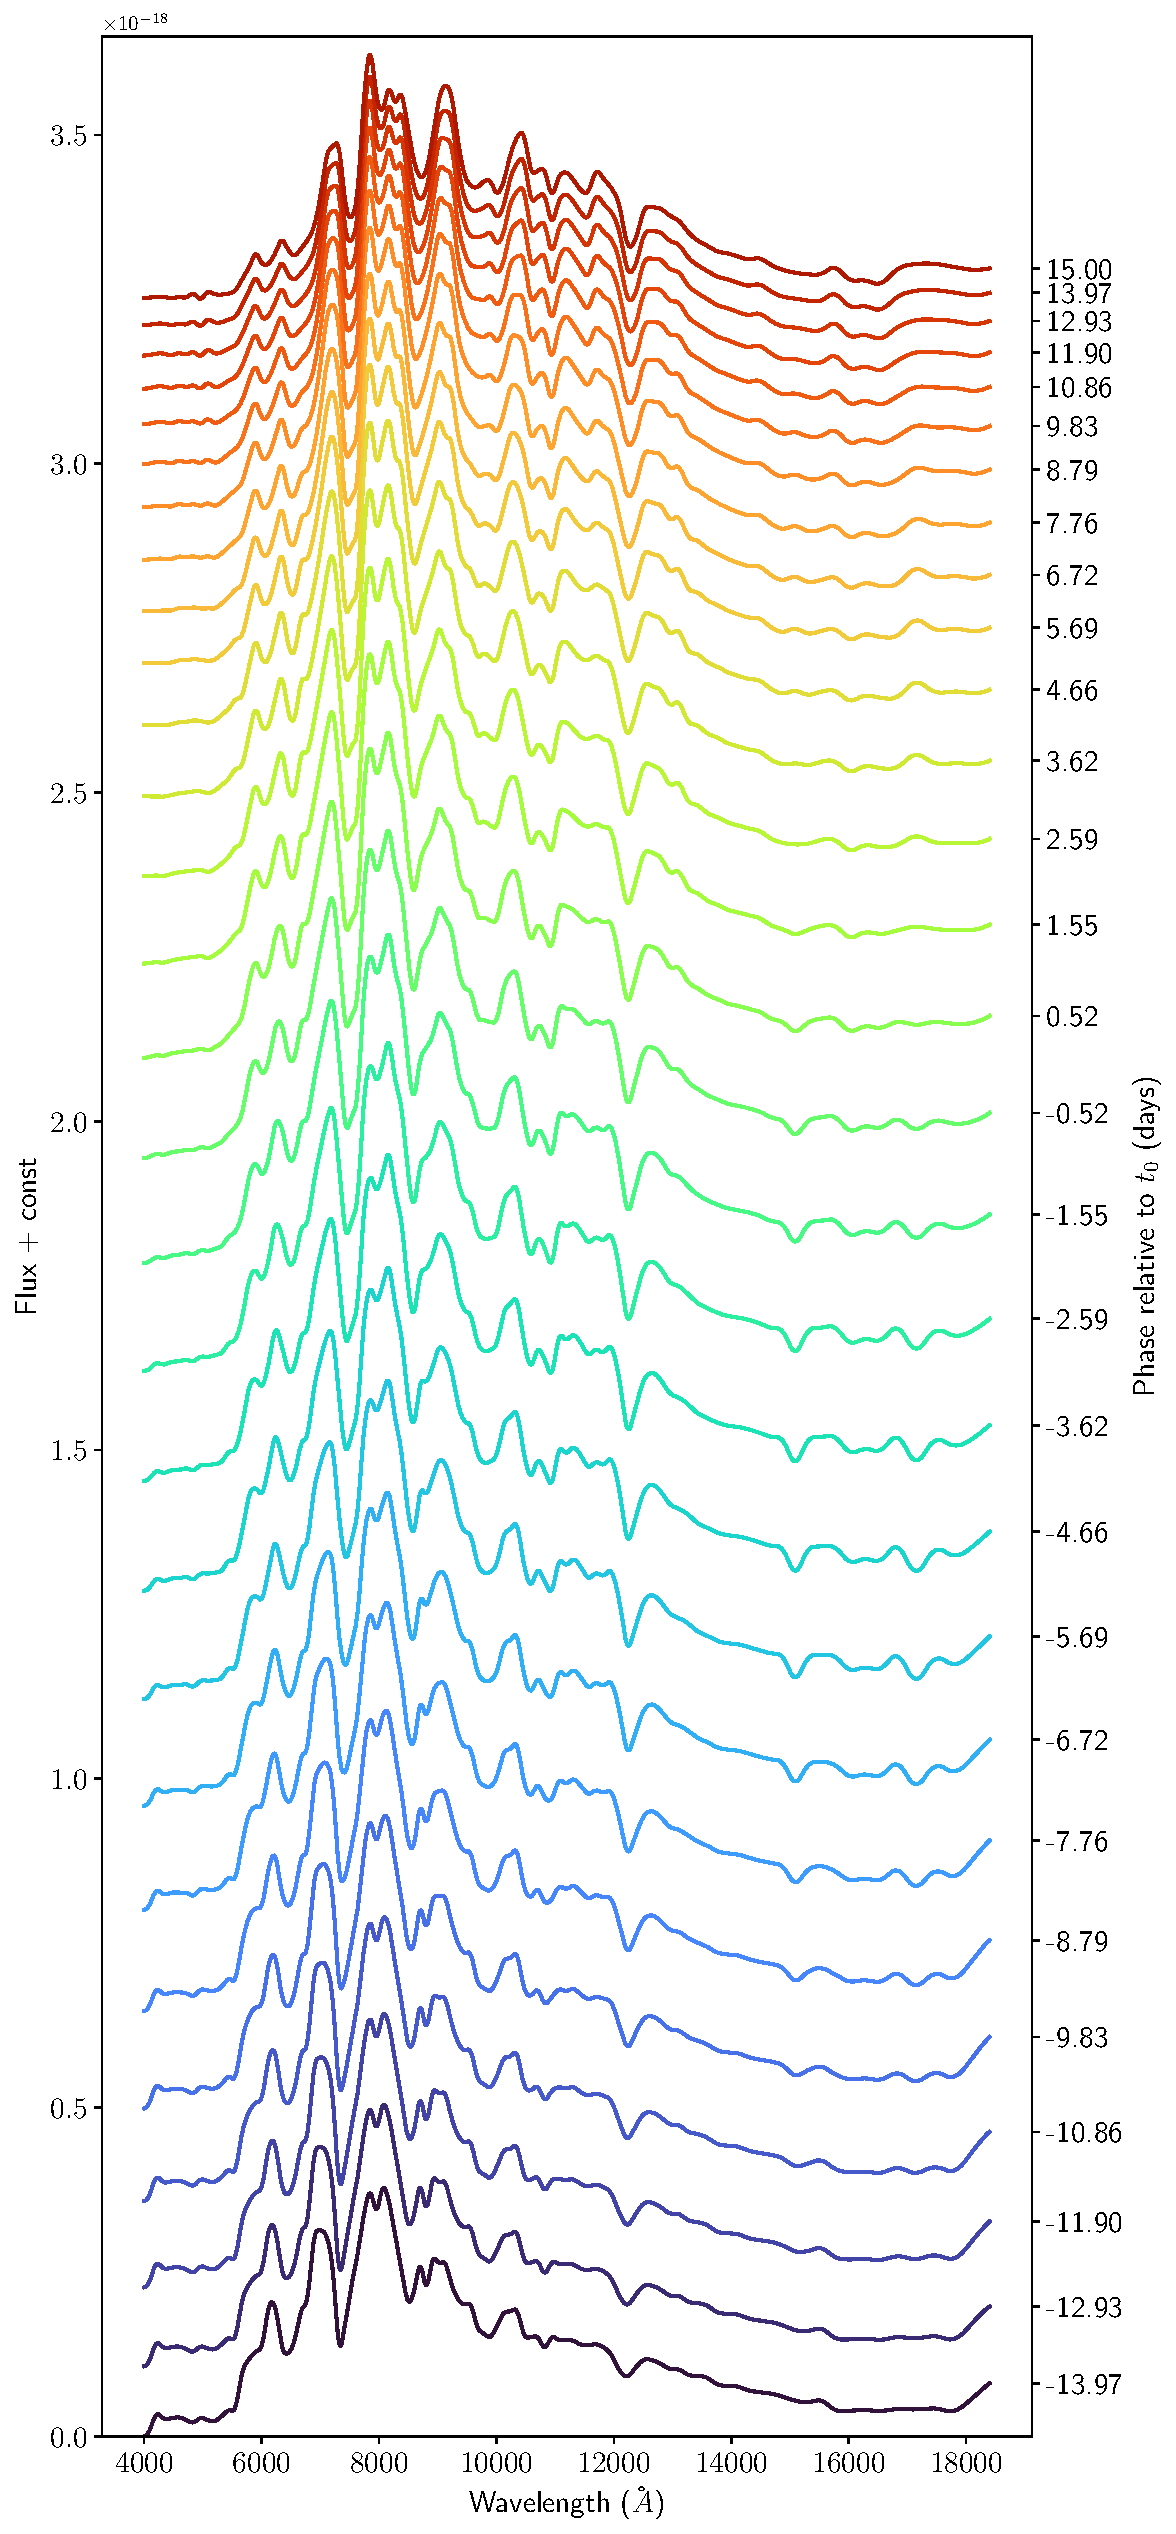
\includegraphics[scale=0.3]{timeseries.pdf}};
        \foreach \d/\y in {x1dist/0.2, cdist/0, zdist/-0.2}{
            \draw[->, >=stealth]
                (\d.east) --
            ([shift={(0,\y)}]TS.west);}
            \coordinate (Tleft) at (TS.east|-TRUE.north east);
            % \node[draw] at (Tleft) {Tleft};
    \end{scope}
    %%%%%%%%%%%%%%%%%%%%%%%%%%%%%%%%%%%%%%%%%%%%%%%%%%%%%%%%%%%%%%%%%%%%%%%
    \begin{pgfonlayer}{background}
        \draw[fill=black!10, rounded corners, ]
            (PRIORBOX.north east |- TRUEBOX.north west) --
            (PRIORBOX.north west |- TRUEBOX.north west) --
            (PRIORBOX.north west |- TRUEBOX.south west) --
            (TRUEBOX.south west -| PRIORBOX.south east) -- cycle ;
    \end{pgfonlayer}
    \begin{pgfonlayer}{background}
        \draw[fill=orchid!20, rounded corners]
            (TRUEBOX.north east) -- (TRUEBOX.north west) --
            (TRUEBOX.south west) -- (TRUEBOX.south east) -- cycle ;
    \end{pgfonlayer}
    %%%%%%%%%%%%%%%%%%%%%%%%%%%%%%%%%%%%%%%%%%%%%%%%%%%%%%%%%%%%%%%%%%%%%%%
    \begin{scope}[local bounding box=SURVEYBOX,
        shift={($(TRUE.east)+(9cm,0)$)}]
        \node[header=cornflowerblue] (SURVEY) at (0,0) {SONDAGE};
        \node[] (TSDSS) at ([shift={(0,-5)}]SURVEY.center)
            {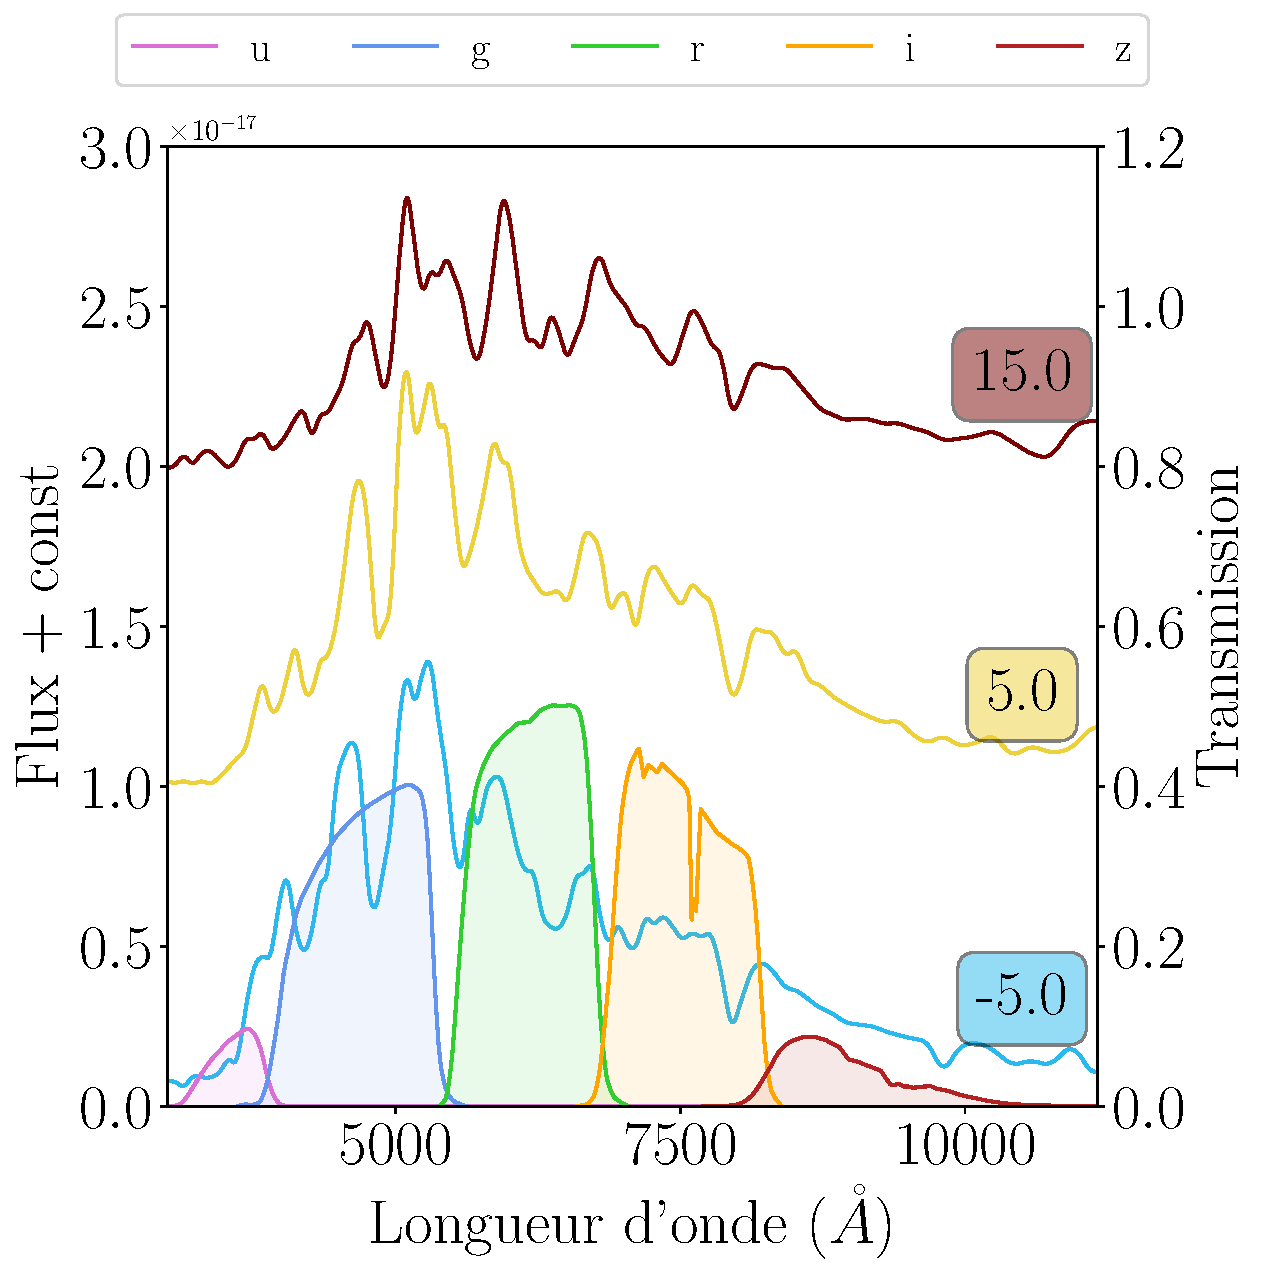
\includegraphics[scale=0.3]{timeseries_sdss.pdf}};
        \node[] (SDLC) at ([shift={(0,-5)}]TSDSS.south)
            {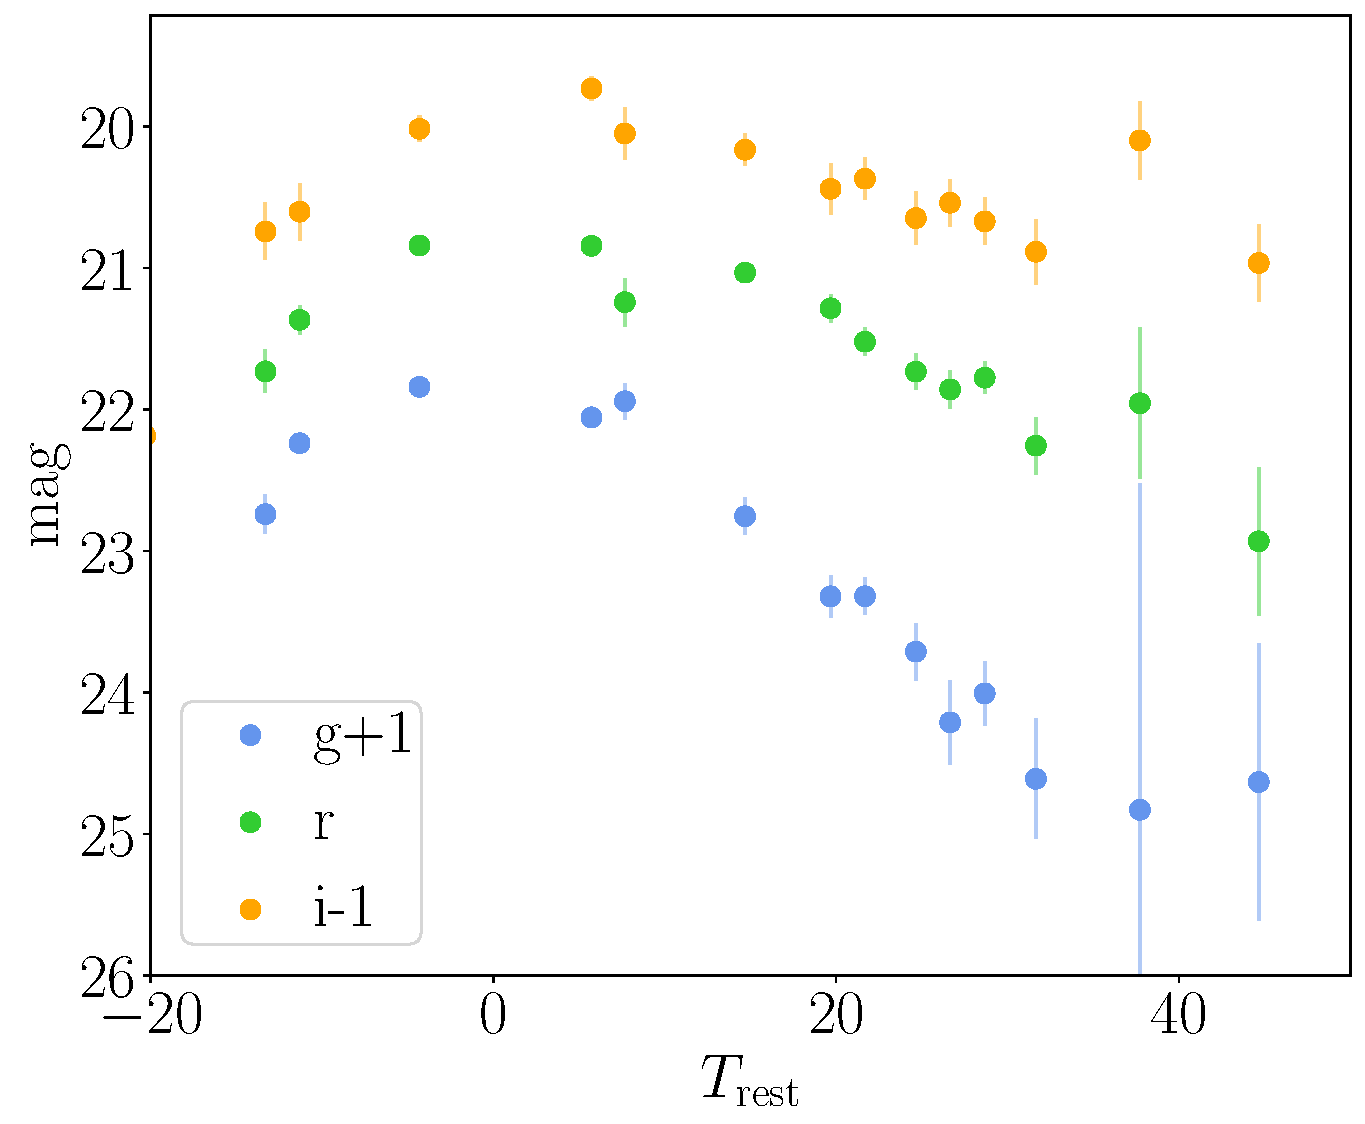
\includegraphics[scale=.5]{lc_2005gg_NOSALT.pdf}};
        \draw[->] (TSDSS.south) -- (SDLC.north);
    \end{scope}
    %%%%%%%%%%%%%%%%%%%%%%%%%%%%%%%%%%%%%%%%%%%%%%%%%%%%%%%%%%%%%%%%%%%%%%%
    \begin{pgfonlayer}{background}
        \draw[fill=cornflowerblue!20, rounded corners]
            (SURVEYBOX.north east) -- (SURVEYBOX.north west) --
            (SURVEYBOX.north west |- TRUEBOX.south west) --
            (TRUEBOX.south east -| SURVEYBOX.south east) -- cycle ;
    \end{pgfonlayer}
    %%%%%%%%%%%%%%%%%%%%%%%%%%%%%%%%%%%%%%%%%%%%%%%%%%%%%%%%%%%%%%%%%%%%%%%
    \begin{scope}[local bounding box=SELECTIONBOX,
        shift={($(SURVEY.east)+(7.9cm,0)$)}]
        % Start SELECTION
        \node[header=limegreen] (SELECTION) at (0,0) {S\'ELECTION};
        % Start PHOTSEL
        \node[header=limegreen]
            (PHOTSEL) at ([shift={(0,-2)}]SELECTION.center) {Photom\'etrique};
        \matrix[matrix of nodes, anchor=north,
            row sep=-1pt, column sep=-\pgflinewidth,
            text width=60pt, align=center,
            %left delimiter=|,
            nodes={anchor=center, align=center}]
            (PHOTLIST) at ([shift={(0,-0.2cm)}]PHOTSEL.south)
            {$T_{\rm rest} < 0$ & $T_{\rm rest} > 10$ & SNR > 5 $gri$ & $\cdots$ \\
            \cmark & \cmark & \xmark \\
            \cmark & \cmark & \xmark \\
            \xmark & \xmark & \cmark \\
            \xmark & \cmark & \xmark \\
            \vdots & \vdots & \vdots \\};
        % Vlines
        \foreach \n in {1, 2, 3}{
        \draw[]
            (PHOTLIST-1-\n.north east-|PHOTLIST-6-\n.south east) |-
        (PHOTLIST-6-\n.south east);}
        % Start SPECSEL
        \node[header=limegreen]
            (SPECSEL) at ([shift={(0,-2)}]PHOTLIST.south) {Spectroscopique};
        %%%%%%%%%%%%%%%%%%%%%%%%%%%%%%%%%%%%%%%%%%%%%%%%%%%%%%%%%%%%%%%%%%%%%%%
        % SDSS SPECEFF from sdss spec
        \pgfplotstableread{../data/sdss_spec.dat}{\sdspectable}
        \findMax{\sdspectable}{r}{\rmax}
        \begin{axis}[name=sdspec, scale=0.8,
            at={(SPECSEL.south west)}, anchor=north west,
            yshift=-1cm, xshift=-1cm,
            xmin=16.0, xmax=\rmax*0.8,
            ymin=0, ymax=1.0,
            xlabel=$r$ (mag), ylabel=\'Efficacit\'e spectroscopique,
            axis lines=left,
            clip=true]
            \addplot[black, smooth]
                table[x=r, y=SPECEFF] from \sdspectable;
        \end{axis}
        % \matrix[matrix of nodes, anchor=north,
        %     row sep=-1pt, column sep=-\pgflinewidth,
        %     text width=40pt, align=center,
        %     %left delimiter=|,
        %     nodes={anchor=center, align=center}]
        %     (SPECLIST) at ([shift={(0,-0.2cm)}]SPECSEL.south)
        %     {$z$ | & Date | & RADEC \\
        %     \vdots & \vdots & \vdots \\};
    \end{scope}
    %%%%%%%%%%%%%%%%%%%%%%%%%%%%%%%%%%%%%%%%%%%%%%%%%%%%%%%%%%%%%%%%%%%%%%%
    \begin{pgfonlayer}{background}
        \draw[fill=limegreen!20, rounded corners]
            (SELECTIONBOX.north east) -- (SELECTIONBOX.north west) --
            (SELECTIONBOX.north west |- TRUEBOX.south west) --
            (TRUEBOX.south east -| SELECTIONBOX.south east) -- cycle ;
    \end{pgfonlayer}
    %%%%%%%%%%%%%%%%%%%%%%%%%%%%%%%%%%%%%%%%%%%%%%%%%%%%%%%%%%%%%%%%%%%%%%%
    \begin{scope}[local bounding box=CONSBOX,
        shift={($(SELECTION.east)+(5cm,0)$)}]
    %%%%%%%%%%%%%%%%%%%%%%%%%%%%%%%%%%%%%%%%%%%%%%%%%%%%%%%%%%%%%%%%%%%%%%%
        % Start CONS
        \node[header=orange] (CONS) at (3,0) {CONSERV\'E};
        %%%%%%%%%%%%%%%%%%%%%%%%%%%%%%%%%%%%%%%%%%%%%%%%%%%%%%%%%%%%%%%%%%%%%%%
        % M DIST from dumps and 2_LCFIT
        \pgfplotstableread{../data/mTrue_SDSS.txt}{\mtrue}
        \pgfplotstableread{../data/mSelected_SDSS.txt}{\msel}
        \pgfplotstableread{../data/mFitted_SDSS.txt}{\mfit}
        \begin{axis}[name=mdump, scale=0.7,
            yshift=-1.5cm, anchor=north west,
            xmin=7, xmax=12.1,
            ymin=0, ymax=0.73,
            xlabel=$M$, ylabel=$P$,
            axis lines=left,
            legend pos=north west,
            clip=false]
            \addplot[smooth, orchid, line width=2pt]
                table[x=mlin, y=values] from \mtrue;
            \addlegendentry{V\'erit\'e}
            \addplot[smooth, limegreen, line width=2pt]
                table[x=mlin, y=values] from \msel;
            \addlegendentry{S\'electionn\'e}
            \addplot[smooth, orange, line width=2pt]
                table[x=mlin, y=values] from \mfit;
            \addlegendentry{Ajust\'e}
        \end{axis}
        %%%%%%%%%%%%%%%%%%%%%%%%%%%%%%%%%%%%%%%%%%%%%%%%%%%%%%%%%%%%%%%%%%%%%%%
        % X1 DIST dumps and 2_LCFIT
        \pgfplotstableread{../data/xTrue_SDSS.txt}{\xtrue}
        \pgfplotstableread{../data/xSelected_SDSS.txt}{\xsel}
        \pgfplotstableread{../data/xFitted_SDSS.txt}{\xfit}
        \begin{axis}[name=xdump, scale=0.7,
            at={(mdump.below south west)},
            yshift=-0.3cm, anchor=north west,
            xmin=-3, xmax=3,
            ymin=0, ymax=0.5,
            xlabel=$x_1$, ylabel=$P$,
            axis lines=left,
            legend pos=north west,
            clip=false]
            \addplot[smooth, orchid, line width=2pt]
                table[x=xlin, y=values] from \xtrue;
            % \addlegendentry{V\'erit\'e}
            \addplot[smooth, limegreen, line width=2pt]
                table[x=xlin, y=values] from \xsel;
            % \addlegendentry{S\'electionn\'e}
            \addplot[smooth, orange, line width=2pt]
                table[x=xlin, y=values] from \xfit;
            % \addlegendentry{Ajust\'e}
        \end{axis}
        %%%%%%%%%%%%%%%%%%%%%%%%%%%%%%%%%%%%%%%%%%%%%%%%%%%%%%%%%%%%%%%%%%%%%%%
        % C DIST dumps and 2_LCFIT
        \pgfplotstableread{../data/cTrue_SDSS.txt}{\ctrue}
        \pgfplotstableread{../data/cSelected_SDSS.txt}{\csel}
        \pgfplotstableread{../data/cFitted_SDSS.txt}{\cfit}
        \begin{axis}[name=cdump, scale=0.7,
            at={(xdump.below south west)},
            yshift=-0.3cm, anchor=north west,
            xmin=-0.3, xmax=0.4,
            ymin=0, ymax=7.2,
            xlabel=$c$, ylabel=$P$,
            axis lines=left,
            legend pos=north west,
            clip=false]
            \addplot[smooth, orchid, line width=2pt]
                table[x=clin, y=values] from \ctrue;
            % \addlegendentry{V\'erit\'e}
            \addplot[smooth, limegreen, line width=2pt]
                table[x=clin, y=values] from \csel;
            % \addlegendentry{S\'electionn\'e}
            \addplot[smooth, orange, line width=2pt]
                table[x=clin, y=values] from \cfit;
            % \addlegendentry{Ajust\'e}
        \end{axis}
        %%%%%%%%%%%%%%%%%%%%%%%%%%%%%%%%%%%%%%%%%%%%%%%%%%%%%%%%%%%%%%%%%%%%%%%
        % Z DIST dumps and 2_LCFIT
        \pgfplotstableread{../data/zTrue_SDSS.txt}{\ztrue}
        \findMax{\ztrue}{zlin}{\zxmax}
        \findMax{\ztrue}{values}{\zymax}
        \pgfplotstableread{../data/zSelected_SDSS.txt}{\zsel}
        \pgfplotstableread{../data/zFitted_SDSS.txt}{\zfit}
        \begin{axis}[name=zdump, scale=0.7,
            at={(cdump.below south west)},
            yshift=-0.3cm, anchor=north west,
            xmin=0, xmax=\zxmax,
            ymin=0, ymax=\zymax,
            xlabel=$z$, ylabel=$P$,
            axis lines=left,
            legend pos=north west,
            clip=false]
            \addplot[smooth, orchid, line width=2pt]
                table[x=zlin, y=values] from \ztrue;
            % \addlegendentry{V\'erit\'e}
            \addplot[smooth, limegreen, line width=2pt]
                table[x=zlin, y=values] from \zsel;
            % \addlegendentry{S\'electionn\'e}
            \addplot[smooth, orange, line width=2pt]
                table[x=zlin, y=values] from \zfit;
            % \addlegendentry{Ajust\'e}
        \end{axis}
        %%%%%%%%%%%%%%%%%%%%%%%%%%%%%%%%%%%%%%%%%%%%%%%%%%%%%%%%%%%%%%%%%%%%%%%
    \end{scope}
    %%%%%%%%%%%%%%%%%%%%%%%%%%%%%%%%%%%%%%%%%%%%%%%%%%%%%%%%%%%%%%%%%%%%%%%
    \begin{pgfonlayer}{background}
        \draw[fill=orange!20, rounded corners]
            (CONSBOX.north east) -- (CONSBOX.north west) --
            (CONSBOX.north west |- TRUEBOX.south west) --
            (TRUEBOX.south east -| CONSBOX.south east) -- cycle ;
    \end{pgfonlayer}
    %%%%%%%%%%%%%%%%%%%%%%%%%%%%%%%%%%%%%%%%%%%%%%%%%%%%%%%%%%%%%%%%%%%%%%%
    % \begin{scope}[shift={(16,0)}]
    %     \node[header=red] (SIMRES) at (0,0) {Simulation propreties};
    % \end{scope}
    % \begin{scope}[shift={(20,0)}]
    %     \node[header=blue] (LCFIT) at (0,0) {LC fit};
    % \end{scope}
\end{tikzpicture}
\end{document}
